\chapter{Special Relativity: Time Dilation}
\label{phys:time-dilation}

\assumes{Pythagoras' theorem; distance $=$ speed $\times$ time; the two postulates of special relativity (stated in the remark at the end).}

\begin{center}
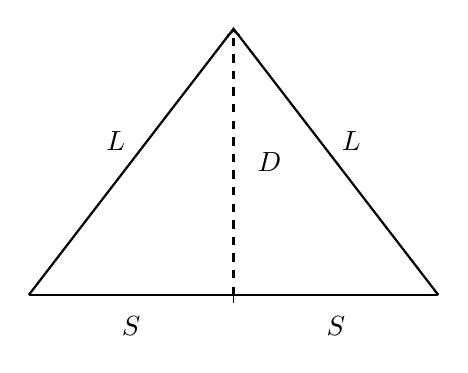
\begin{tikzpicture}[scale=1.3]
    % Coordinates
    \coordinate (A) at (-2,0);   % base left
    \coordinate (B) at (2,0);    % base right
    \coordinate (M) at (0,0);    % base midpoint
    \coordinate (T) at (0,2.6);  % apex

    % Triangle sides (path of light on the moving ship, as seen from Earth)
    \draw[thick] (A) -- (T) -- (B);
    \draw[thick] (A) -- (B);

    % Dashed height (path of light as seen on the ship)
    \draw[dashed, thick, ->] (M) -- (T);

    % Labels for the slanted sides
    \node at (-1.15,1.5) {$L$};
    \node at (1.15,1.5) {$L$};

    % Label for height
    \node at (0.35,1.3) {$D$};

    % Tick mark showing midpoint of base
    \draw (0,-0.08) -- (0,0.08);

    % Labels for base segments
    \node at (-1,-0.3) {$S$};
    \node at (1,-0.3) {$S$};
\end{tikzpicture}
\end{center}

\noindent
\textbf{Setup:}
\begin{align*}
2D &= ct       &&\therefore D = \frac{ct}{2}     &&\text{(light's path, observer on ship)}\\
2S &= v t_0    &&\therefore S = \frac{v t_0}{2}  &&\text{(ship's speed, observer on Earth)}\\
2L &= c t_0    &&\therefore L = \frac{c t_0}{2}  &&\text{(light's path, observer on Earth)}
\end{align*}

\noindent
\textbf{Pythagorean relation:}
\[
L^2 = D^2 + S^2
\]

\noindent
\textbf{Substituting:}
\begin{align*}
\left(\frac{c t_0}{2}\right)^2 &= \left(\frac{ct}{2}\right)^2 + \left(\frac{v t_0}{2}\right)^2 \\[6pt]
\frac{c^2 t_0^2}{4} &= \frac{c^2 t^2}{4} + \frac{v^2 t_0^2}{4} \\[6pt]
\therefore\; c^2 t_0^2 &= c^2 t^2 + v^2 t_0^2 \\[6pt]
c^2 t_0^2 - v^2 t_0^2 &= c^2 t^2 \\[6pt]
\frac{c^2 t_0^2 - v^2 t_0^2}{c^2} &= t^2 \\[6pt]
t_0^2 \left(1 - \frac{v^2}{c^2}\right) &= t^2 \\[6pt]
\sqrt{t_0^2} &= \sqrt{\dfrac{t^2}{1 - \dfrac{v^2}{c^2}}} \\[6pt]
\therefore\; t_0 &= \frac{t}{\sqrt{1 - \dfrac{v^2}{c^2}}}
\end{align*}
\begin{center}
\boxed{\therefore\; t_0 = \frac{t}{\sqrt{1 - \dfrac{v^2}{c^2}}}}
\end{center}

\bigskip
\noindent\textbf{Remark.} The factor $1/\sqrt{1-v^2/c^2}$ that shows up here is important enough to have its own symbol, $\gamma$, called the \emph{Lorentz factor} -- named after Hendrik Lorentz, who worked out very similar mathematics years before Einstein published special relativity in 1905, originally to explain the null result of the Michelson--Morley experiment. It's worth looking at the two extremes: for everyday speeds ($v \ll c$), $\gamma \approx 1$ and $t_0 \approx t$, which is exactly why nobody notices time dilation in ordinary life; but as $v \to c$, $\gamma \to \infty$, so a clock moving at (nearly) the speed of light appears, to an outside observer, to almost stop. What makes this especially striking is how little was assumed to derive it: just that the laws of physics look the same in every inertial frame, and that the speed of light $c$ is the same for \emph{every} observer, no matter how fast the light source is moving -- two simple postulates producing a deeply counter-intuitive conclusion.
